\documentclass[12pt]{article}
\usepackage{amsmath}
\usepackage{mathtools}
\usepackage{graphicx}
\usepackage{float}
\begin{document}
\title{Electrical Engineering 141, Final Project Report}
\date{March 14th, 2019}
\author{Michael Wu\\UID: 404751542}
\maketitle

\section{Current Control Loop Design}

\paragraph{a)}

Consider the relationship between \(V_a\) and \(V_c\). The voltage at the negative
terminal of the OpAmp is \(\frac{V_a}{5}\). Then we can solve the following equation.
\begin{align*}
    V_a&=k\left(V_c-\frac{V_a}{5}\right)\\
    V_a&=\frac{5k}{5+k}V_c\\
    V_a&=5V_c
\end{align*}

Next consider the relationship between \(V_s\) and \(I_c\). Since \(R_s\) is very low,
we can assume all the current flows through \(R_s\). Then the voltage at the positive input of the
OpAmp is \(\frac{5}{6}I_cR_s\). Since \(R_s=0.2\) this just becomes \(\frac{I_c}{6}\).
The voltage at the negative input of the OpAmp is \(\frac{V_s}{6}\).
We then have the following relationship.
\begin{align*}
    V_s&=\frac{k}{6}(I_c-V_s)\\
    V_s&=\frac{k}{6+k}I_c\\
    V_s&=I_c
\end{align*}

Now consider the term \(x^\prime\). This has a Laplace transform of \(sX\).
From the mechanical behavior of the FTS, we obtain the following equation.
\begin{align*}
    s^2m_1X &= K_fI_c - sb_1X - k_1X\\
    X&=\frac{K_f}{m_1s^2 + b_1s + k_1}I_c\\
    sX&=\frac{K_fs}{m_1s^2 + b_1s + k_1}I_c
\end{align*}
Then using \(I_c\) and \(V_a\) we can then solve the following relationship.
\begin{align*}
    I_c (R_c + R_s + sL_c) &= V_a - K_f sX\\
    I_c (R_c + R_s + sL_c) &= V_a - \frac{K_f^2s}{m_1s^2 + b_1s + k_1}I_c\\
    I_c &=\frac{m_1s^2 + b_1s + k_1}{(m_1s^2 + b_1s + k_1)(R_c + R_s + sL_c)+K_f^2s}V_a\\
    V_s &= \frac{5(m_1s^2 + b_1s + k_1)}{(m_1s^2 + b_1s + k_1)(R_c + R_s + sL_c)+K_f^2s}V_c\\
    P_{elec} &= \frac{5(m_1s^2 + b_1s + k_1)}{(m_1s^2 + b_1s + k_1)(4.2 + 0.0002s)+K_f^2s}
\end{align*}

\paragraph{b)}

If the back emf is zero, then we can obtain the following equation instead.
\begin{align*}
    I_c (R_c + R_s + sL_c) &= V_a\\
    I_c &=\frac{1}{R_c + R_s + sL_c}V_a\\
    V_s &= \frac{5}{R_c + R_s + sL_c}V_c\\
    P_{elec} &= \frac{5}{4.2 + 0.0002s}
\end{align*}

\paragraph{c)}

At high frequencies, these are equal because the \(s^2\) term will dominate the transfer
function with back emf included. Then only the coefficient \(5m_1\) in the numerator and
\((4.2 + 0.0002s)m_1\) in the denominator will have an effect on the transfer function.
Thus we obtain the following transfer function.
\[P_{elec} \approx \frac{5m_1}{(4.2 + 0.0002s)m_1} = \frac{5}{4.2 + 0.0002s}\]
This is exactly the same as the transfer function with no back emf. The physical reason
this happens is because as the frequency increases beyond the resonant frequency, the FTS
dynamics will cause the position and velocity of the FTS to become smaller and smaller.

\paragraph{d)}

The components \(R_3\), \(C_1\), and \(C_2\) form an equivalent component with the following
impedance.
\[Z=\frac{C_1R_3s + 1}{s(C_1C_2R_3s + C_1 + C_2)}\]
We can assume the input to the negative terminal of the OpAmp is zero. Then we can write
the following equations.
\begin{align*}
    \frac{V_c}{Z}&=-\frac{V_s}{R_2}\\
    -\frac{V_c}{V_s}&=\frac{Z}{R_2}\\
    C_{elec} &=\frac{C_1R_3s + 1}{R_2s(C_1C_2R_3s + C_1 + C_2)}
\end{align*}
The transfer function between \(V_c\) and \(V_{set}\) is exactly the same
except the sign is flipped and \(R_2\) is replaced by \(R_1\). Since
\(V_c=C_{elec}H_{V_{set}V_r}V_{set}\), we then know that \(H_{V_{set}V_r}=-\frac{R_2}{R_1}\).
The overall closed loop transfer function is shown below.
\[H_{V_{set}I_c}=H_{V_{set}V_r}\frac{C_{elec}P_{elec}}{1+C_{elec}P_{elec}}\]
Note that as \(s\) becomes very small, the open loop transfer function will go to infinity due to the
root at zero. In the closed loop transfer function, this means that both the numerator and denominator
of the fractional term will grow at the same rate. This leads to a limit of one as \(s\) goes to zero.
Then with the steady state gain condition we can use the final value theorem to write the following equation.
\begin{align*}
    5&=\lim_{s\to 0} s\frac{-10}{s}H_{V_{set}V_r}\frac{C_{elec}P_{elec}}{1+C_{elec}P_{elec}}\\
    &=10\frac{R_2}{R_1}\\
    R_2&=5000
\end{align*}
If we let \(s=(6\times 10^5)j\), we can then use the gain crossover and phase margin conditions to solve for
the remaining component values. The value of the plant is the following.
\[P_{elec}=\frac{5}{4.2 + 0.0002\times6\times 10^5j}=0.04164116925e^{j\frac{\pi}{180}(-87.9955)}\]
The value of the controller is the following.
\begin{align*}
    C_{elec} &=\frac{C_1R_3(6\times 10^5)j + 1}{5000(6\times 10^5)j(C_1C_2R_3(6\times 10^5)j + C_1 + C_2)}\\
    &=\frac{1}{3\times10^9}\frac{1+jC_1R_3(6\times 10^5)}{-C_1C_2R_3(6\times 10^5)+j(C_1+C_2)}
\end{align*}
We want the gain to be 1 at this frequency so we obtain the following equation.
\begin{align*}
    \frac{0.04164116925}{3\times10^9}\sqrt{\frac{C_1^2R_3^2(6\times 10^5)^2 + 1}{C_1^2C_2^2R_3^2(6\times 10^5)^2 + (C_1+C_2)^2}} &=1\\
    \sqrt{\frac{C_1^2R_3^2(6\times 10^5)^2 + 1}{C_1^2C_2^2R_3^2(6\times 10^5)^2 + (C_1+C_2)^2}}&=\frac{3\times10^9}{0.04164116925}
\end{align*}
From the phase margin we obtain the following equation.
\begin{align*}
    \theta &= \tan^{-1}(C_1R_3(6\times 10^5))-90-\tan^{-1}\left(\frac{C_1C_2R_3(6\times 10^5)}{C_1+C_2}\right)-87.9955\\
    \theta &= \tan^{-1}(C_1R_3(6\times 10^5))-\tan^{-1}\left(\frac{C_1C_2R_3(6\times 10^5)}{C_1+C_2}\right) > 60
\end{align*}
Assume that the following conditions hold.
\begin{align*}
    C_1 &\gg C_2\\
    C_1R_3(6\times 10^5) &\gg 1\\
    C_2R_3(6\times 10^5) &\ll 1
\end{align*}
Then the first term will be near 90 and the second term will be near zero which meets our phase requirements.
Lets assume \(C_1R_3 = \frac{1}{6} \times 10^{-4}\) and \(C_1 = 100C_2\). Then we can reduce the gain
equation to obtain the following result.
\begin{align*}
    \sqrt{\frac{10^2 + 1}{C_2^210^2 + (C_1 + C_2)^2}}&=\frac{3\times10^9}{0.04164116925}\\
    \sqrt{\frac{101}{C_2^2(10^2+101^2)}}&=\frac{3\times10^9}{0.04164116925}\\
    \frac{1}{C_2}&=\sqrt{\frac{10^2+101^2}{101}}\frac{3\times10^9}{0.04164116925}\\
    C_2&=\sqrt{\frac{101}{10^2+101^2}}\frac{0.04164116925}{3\times10^9}\\
    &=1.374430089\times 10^{-12}
\end{align*}
By substituting into previous conditions we then get \(C_1=1.374430089\times 10^{-10}\) and \(R_3=1.212623821\times10^5\).

\paragraph{e)}

Here we see that the gain crossover frequency at \(6\times10^5\) and the gain margin greater than \(60\) degrees.
\begin{figure}[H]
    \begin{center}
        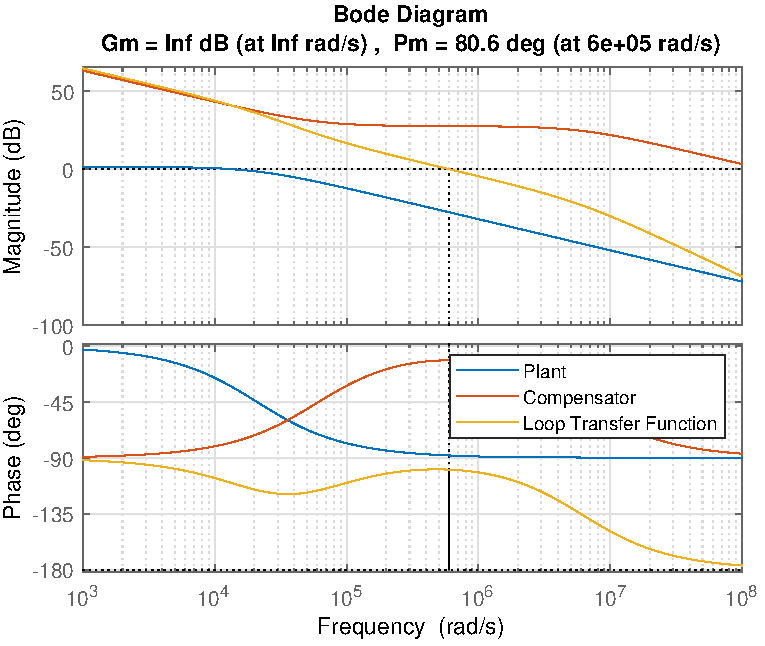
\includegraphics[width=3.5in]{CurrentControl-e.pdf}
    \end{center}
\end{figure}

\section{FTS Plant System Identification}

\paragraph{a)}

From before we have the relationship between \(F\) and \(X\) given by the following equation.
\[X=\frac{1}{m_1s^2 + b_1s + k_1}F\]
If we convert this transfer function into the standard second order form we obtain the following result.
\begin{align*}
    K\frac{\omega^2}{s^2+2\zeta\omega s + \omega^2}&=\frac{1}{m_1s^2 + b_1s + k_1}\\
    &=\frac{1}{m_1}\frac{1}{s^2 + \frac{b_1}{m_1}s + \frac{k_1}{m_1}}\\
    &=\frac{1}{k_1}\frac{\frac{k_1}{m_1}}{s^2 + \frac{b_1}{m_1}s + \frac{k_1}{m_1}}\\
    K=\frac{1}{k_1}\qquad \omega&=\sqrt{\frac{k_1}{m_1}}\qquad\zeta=\sqrt{\frac{m_1}{k_1}}\frac{b_1}{2m_1}
\end{align*}
From visual inspection our DC gain is \(-80\) so we have \(K=10^{-4}\). The corner frequency is \(\omega=10^3\).
The maximum frequency response is \(20\) decibels above the DC gain, so we have \(\zeta=0.05\). Then we obtain
the following constants.
\[k_1=10000 \qquad m_1=0.01 \qquad b_1=1\]

\paragraph{b)}

Since the frequency response had a slope of \(-40\) at the end, I know that there are two more poles than zeros.
I estimated that the time delay was \(10^{-5}\) seconds, since the phase starts decreasing after \(\omega=10^5\).
Then I tested various numbers of poles and zeros to obtain the following code for the plant.
\begin{verbatim}
Gp = tfest(frd(Gpmag.*exp(1j*Gpphase*pi/180),ww),10,8,0.00001);
\end{verbatim}
This exactly matches the given frequency and phase response for the plant.
\begin{figure}[H]
    \begin{center}
        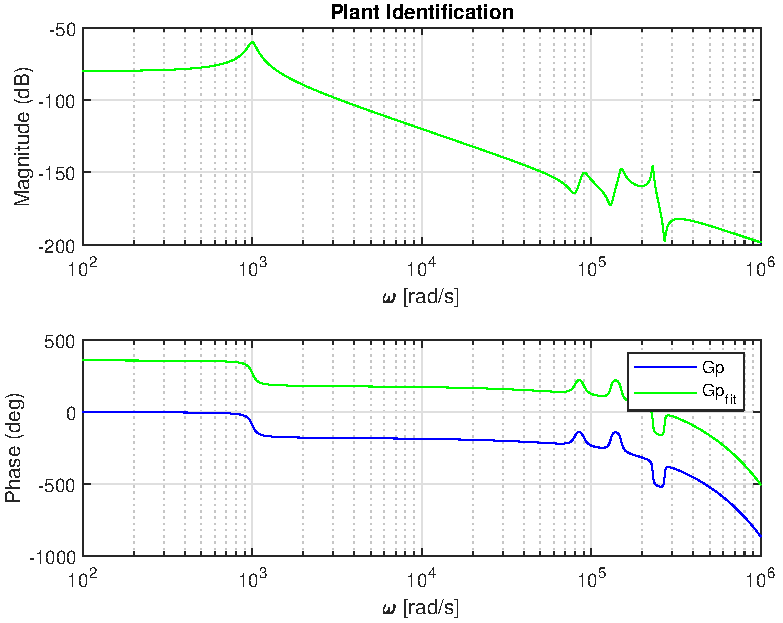
\includegraphics[width=3.5in]{Plant-b.pdf}
    \end{center}
\end{figure}

\section{Position Control Loop Design}

\paragraph{a)}

Let's ignore the noise and obtain the transfer function from the input to the output. It is the following expression.
\[H = \frac{G_1C_{mech}G_aK_fG_p}{1+G_1C_{mech}G_aK_fG_p}\]
We can simplify this by letting \(C^\prime_{mech}=G_1G_aK_fC_{mech}\). Then this becomes
\[H = \frac{C^\prime_{mech}G_p}{1+C^\prime_{mech}G_p}\]
and we only need to worry about the design for \(C^\prime_{mech}\).

In order for the steady state position tracking error to be almost fully eliminated, we want the gain to
become very high as the frequency on the bode plot goes to zero. This can be achieved by adding a pole at \(s=0\).
I will add a \(\frac{s}{10}+1\) term in the numerator to counteract this after the cutoff frequency of \(\omega=10\).

In order for the steady-state position tracking error for the sinusoid to be minimized, we want the gain to be very
high near a frequency of \(\omega=3000\). In order for the noise to have very little effect on the output, we want the gain
to be very low near a frequency of \(\omega=100000\). Based on these requirements, I added two lead compensators with
cutoff frequencies at \(\omega=300\) and \(\omega=3000\). This way we have the maximum difference between the gains at these
two frequencies while still preserving stability. So we have a compensator in the following form.
\[C^\prime_{mech}=K\frac{\frac{s}{10}+1}{s}\left(\frac{\frac{s}{300}+1}{\frac{s}{3000}+1}\right)^2\]
Using the bode plot of the sensitivity function I found that I could set a maximum of \(K=1.3231\times 10^5\) while still
keeping sensitivity below \(10\) dB. For the actual controller I would need to divide by \(G_1G_aK_f=-5\times 10^6\) to
obtain the following gain.
\[K=\frac{1.3231\times10^5}{-5\times 10^6}=-0.026462\]
Then I have the following controller.
\[C_{mech}=-0.026462\frac{\frac{s}{10}+1}{s}\left(\frac{\frac{s}{300}+1}{\frac{s}{3000}+1}\right)^2\]

\paragraph{b)}

The closed loop step response is shown below.
\begin{figure}[H]
    \begin{center}
        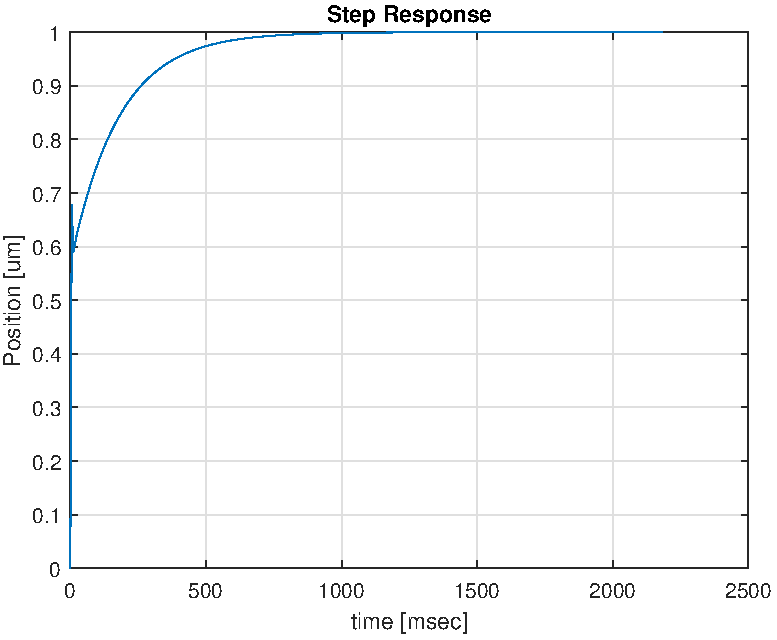
\includegraphics[width=3.5in]{PositionControl-Step.pdf}
    \end{center}
\end{figure}
The transient response characteristics are shown below.
\begin{verbatim}
    RiseTime: 1.3763e-04
SettlingTime: 0.5475
 SettlingMin: 0.5896
 SettlingMax: 1.5025
   Overshoot: 50.2477
  Undershoot: 3.4196e-04
        Peak: 1.5025
    PeakTime: 2.8863e-04
\end{verbatim}
This overshoot is quite large. However, it is not easy to see in the step response graph because it dies out
very fast. I could have designed the controller with a smaller overshoot but that was not one of my design goals. I could
reduce it by reducing the gain, but that would mean that the tracking of the sinusoid input would become worse. It
would increase the settling time. The noise error and sine response are shown below.
\begin{figure}[H]
    \begin{center}
        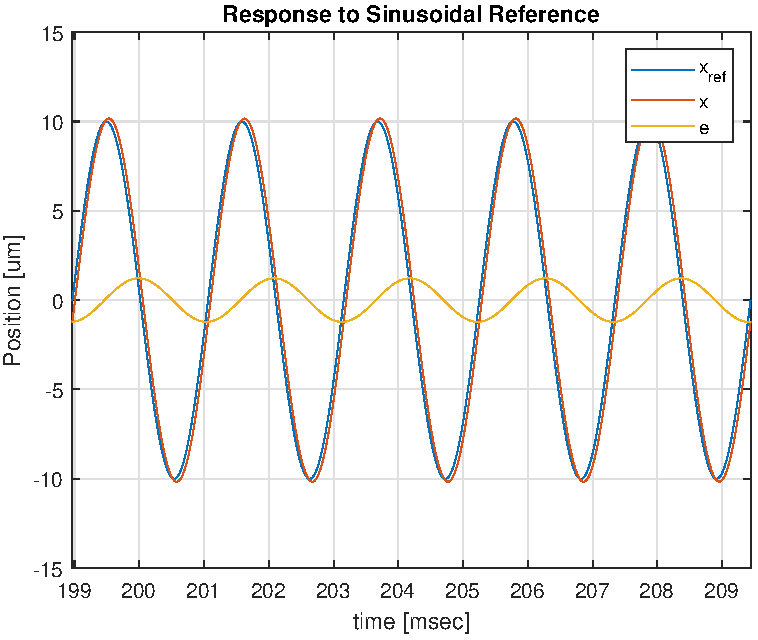
\includegraphics[width=3.5in]{PositionControl-Sine.pdf}
    \end{center}
\end{figure}
\begin{figure}[H]
    \begin{center}
        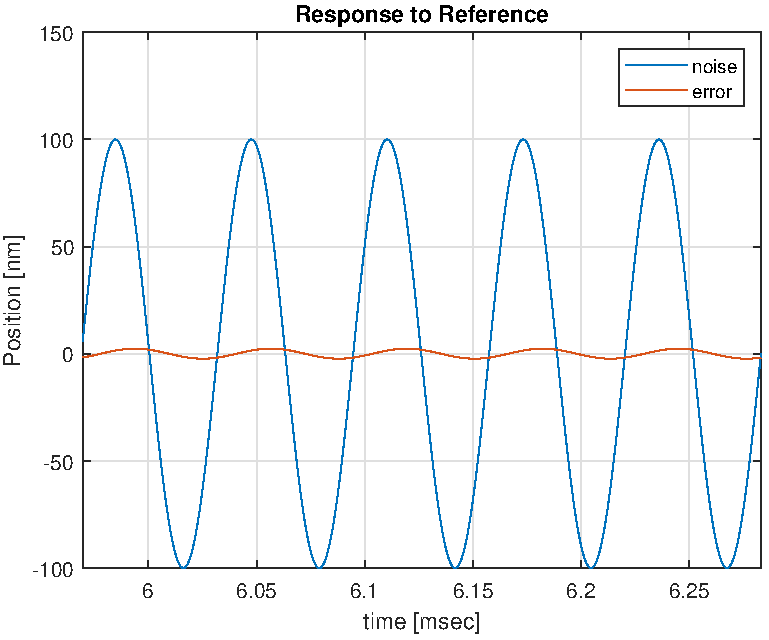
\includegraphics[width=3.5in]{PositionControl-Noise.pdf}
    \end{center}
\end{figure}

\paragraph{c)}

The Bode, Nyquist, and Sensitivity plots are shown below.
\begin{figure}[H]
    \begin{center}
        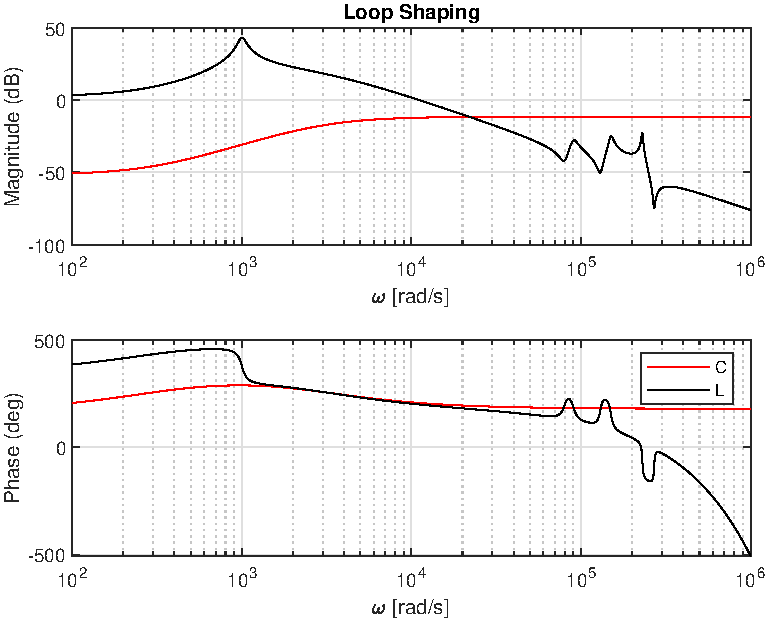
\includegraphics[width=3.5in]{PositionControl-Bode.pdf}
    \end{center}
\end{figure}
\begin{figure}[H]
    \begin{center}
        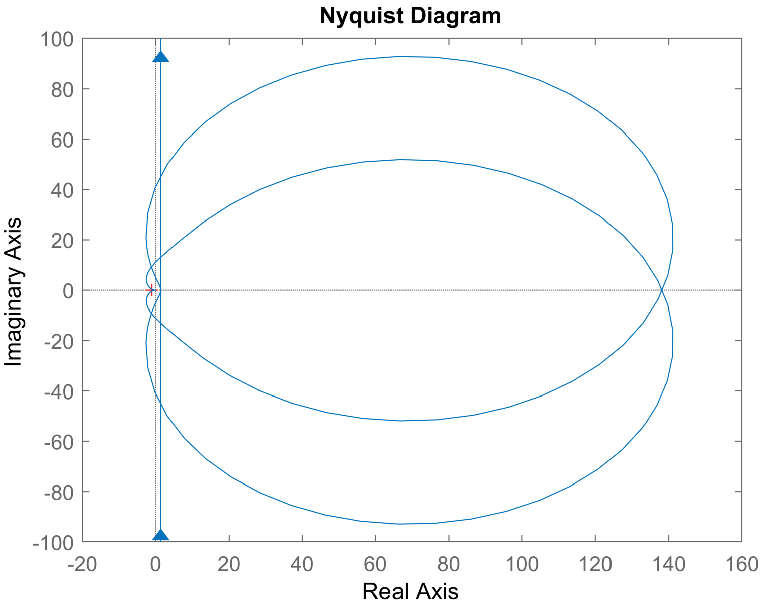
\includegraphics[width=3.5in]{PositionControl-Nyquist.pdf}
    \end{center}
\end{figure}
\begin{figure}[H]
    \begin{center}
        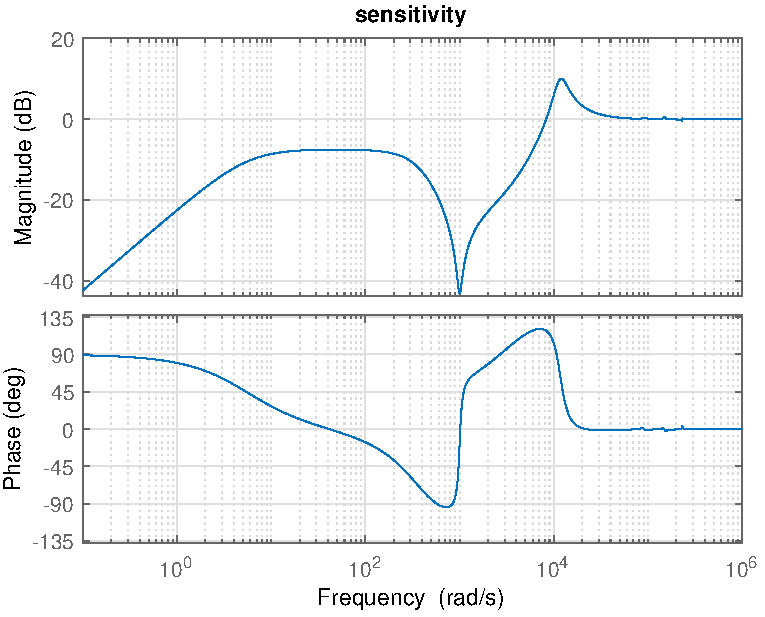
\includegraphics[width=3.5in]{PositionControl-Sensitivity.pdf}
    \end{center}
\end{figure}
Here we can tell that the system is stable from the Bode plot since the gain is negative
at the phase crossover frequency and the phase is above \(-180\) at the gain crossover
frequency.

\end{document}